\documentclass[10pt,a4paper]{article}

% --- Pacotes Essenciais ---
\usepackage[utf8]{inputenc} % Codificação de entrada
\usepackage[T1]{fontenc}    % Codificação da fonte
\usepackage[portuguese]{babel} % Idioma
\usepackage{amsmath, amssymb} % Símbolos matemáticos
\usepackage{graphicx}     % Inclusão de imagens
\usepackage{xcolor}
\usepackage{multicol}     % Múltiplas colunas
\usepackage{geometry}     % Configuração de margens
\usepackage{fancyhdr}     % Cabeçalhos e rodapés personalizados
\usepackage{listings}     % Formatação de código fonte
\usepackage{float}        % Melhor controle de flutuantes (figuras, tabelas)
\usepackage{caption}      % Melhor controle de legendas
\usepackage{booktabs}     % Tabelas com melhor visual
\usepackage{siunitx}      % Alinhamento de números em tabelas
\usepackage{hyperref}     % Links (opcional, mas útil)
% \usepackage{lipsum} % Remover se não precisar mais de texto de exemplo

% --- Configuração de Geometria ---
% Margens reduzidas, headheight para fancyhdr, headsep para espaço abaixo do header
\geometry{left=1cm, right=1cm, top=1.2cm, bottom=1.2cm, headheight=14pt, headsep=8pt}

% --- Configuração do Cabeçalho (fancyhdr) ---
\pagestyle{fancy}
\fancyhf{} % Limpa cabeçalho e rodapé atuais
\fancyhead[L]{} % Sem nome de grupo
\fancyhead[R]{Paralelização OpenMP: Validação Merkle} % Cabeçalho direito
\fancyfoot[C]{\thepage} % Número da página no centro do rodapé
\renewcommand{\headrulewidth}{0.4pt} % Linha separadora do cabeçalho

% --- Configuração do Listings (Código Fonte) ---
\lstdefinestyle{customc}{
language=C,
basicstyle=\footnotesize\ttfamily,
keywordstyle=\color{blue},
commentstyle=\color{green!60!black},
stringstyle=\color{red},
numbers=left,
numberstyle=\tiny\color{gray},
stepnumber=1,
numbersep=5pt,
backgroundcolor=\color{gray!10},
showspaces=false,
showstringspaces=false,
showtabs=false,
frame=single,
rulecolor=\color{black},
tabsize=2,
captionpos=b,
breaklines=true,
breakatwhitespace=true,
postbreak=\mbox{\textcolor{red}{$\hookrightarrow$}\space},
escapeinside={\%*}{*)},
morekeywords={omp_get_wtime}
}
\lstset{style=customc}

% --- Configuração siunitx ---
\sisetup{
output-decimal-marker={,},
table-format = 1.6,
round-mode = places,
round-precision = 6,
}

% --- Informações do Documento ---
\title{Relatório de Paralelização OpenMP \\ Validação de Árvore de Merkle}
\author{Daniel Cierco e Bruno Mossmann}
\date{\today}

% --- Início do Documento ---
\begin{document}

% --- Primeira Página: Duas Colunas ---
\twocolumn[
\begin{@twocolumnfalse} % Ambiente para manter título/autor em coluna única
    \maketitle
    \thispagestyle{fancy} % Aplica o estilo fancyhdr na primeira página
\end{@twocolumnfalse}
]
% Reduzir espaço após o título
\vspace{-2em}

% --- Conteúdo da Primeira Página ---
\section*{Introdução}
Este relatório detalha a paralelização, usando OpenMP, de um algoritmo de validação baseado em Árvore de Merkle. O foco é a aplicação das diretivas e a análise de desempenho (speedup) obtido em um cluster (LAD) e em uma máquina local (M3 Pro).

\section*{O Problema: Validação com Árvores de Merkle}
Árvores de Merkle são estruturas de dados criptográficas usadas para verificar eficientemente a integridade de grandes conjuntos de dados. Os dados são divididos em blocos, cada um sendo hasheado (folhas da árvore). Pares de hashes são concatenados e hasheados recursivamente, formando nós internos, até que um único hash raiz (Merkle Root) represente todo o conjunto.

A \textbf{validação} de um bloco específico não requer o conjunto de dados inteiro. Necessita-se apenas do bloco (ou seu hash), da Merkle Root conhecida e de uma "Prova Merkle" (Merkle Proof): a lista ordenada dos hashes irmãos no caminho da folha até a raiz. O processo envolve recomputar o hash no caminho ascendente, combinando o hash atual com o próximo hash da prova e hasheando o resultado iterativamente. Se a raiz calculada final for igual à Merkle Root conhecida, o bloco é válido. A carga computacional principal está nas operações de hash repetidas.

\subsection*{Potencial de Paralelização}
O gargalo surge ao validar \textit{muitos} blocos diferentes (cada um com sua prova) contra a mesma Merkle Root. Como cada validação é totalmente independente, elas podem ser executadas em paralelo. Se houver $N_{val}$ validações e $P$ processadores/threads, cada thread pode, idealmente, realizar $N_{val}/P$ validações concorrentemente.

\section*{Metodologia}
O processo seguiu os passos:
\begin{enumerate} \itemsep0pt \parskip0pt
    \item \textbf{Baseline:} Medição do tempo sequencial ($T_{seq}$) em 1 core do LAD para datasets \texttt{data8} a \texttt{data80000}.
    \item \textbf{Paralelização:} Uso da diretiva \texttt{\#pragma omp parallel for} no laço C que itera sobre as $N_{val}$ validações independentes. O escalonamento \texttt{schedule(static)} (padrão ou explícito) foi considerado adequado pela natureza uniforme do trabalho por iteração.
    \item \textbf{Execuções:} Medição do tempo paralelo ($T_{par}(N)$) com \texttt{omp\_get\_wtime()}, variando o número de threads $N \in \{1, 2, 4, 8, 16\}$. Executado no LAD (nodo \texttt{--exclusive}) e na máquina local (Apple M3 Pro 12c/18GB, macOS 15.5).
    \item \textbf{Métricas e Plotagem:} Para avaliar o ganho de desempenho com $N$ threads, calculou-se o \textbf{Speedup} $S(N) = T_{seq} / T_{par}(N)$ e a \textbf{Eficiência} $E(N) = S(N) / N$. Os resultados de speedup foram plotados (ver Apêndice B). Um $S(N)=N$ (ou $E(N)=1$) representa o ganho ideal.
\end{enumerate}

\section*{Resultados e Análise Concisa}
Tempos exatos no Apêndice A, gráficos no Apêndice B.

\textbf{Cluster LAD:} Speedup significativo ($S>1$) para datasets grandes (e.g., Fig. \ref{fig:speedup_data80000}), com $S$ próximo do ideal $N$ para $N=2, 4$. O ganho continua para $N=8, 16$, mas $E$ decresce devido a overheads. Para datasets pequenos (Fig. \ref{fig:speedup_data8}, \ref{fig:speedup_data800}), $S < 1$ (slowdown), pois o overhead supera o pequeno $T_{seq}$, destacando a importância da granularidade.

\textbf{Máquina Local (M3 Pro):} Desempenho consistentemente inferior ao LAD (Apêndice B), com $S \approx 1$ ou $S < 1$ para $N>1$. Arquitetura/ambiente local menos propícia para paralelização sustentada comparada ao cluster.

\textbf{Escalabilidade:} Boa escalabilidade forte no LAD para problemas grandes; pobre na máquina local.

\section*{Conclusão}
A paralelização OpenMP da validação Merkle usando \texttt{\#pragma omp parallel for} é eficaz em hardware adequado (LAD) quando a granularidade (volume de validações) é suficiente. A comparação LAD vs. M3 Pro mostra a sensibilidade à plataforma. OpenMP simplifica a exploração do paralelismo de dados inerente ao problema.

% --- Fim da Primeira Página e mudança para coluna única ---
\onecolumn
\clearpage

% --- Apêndices ---
\appendix
\renewcommand{\thesection}{\Alph{section}}

\section{Dados de Tempo de Execução}
\label{app:dados}

% --- Tabelas de Dados ---
\begin{table}[H]
    \centering
    \caption{Tempos de Execução Sequencial (em segundos).}
    \label{tab:seq_times}
    \begin{tabular}{l S[table-format=1.6] S[table-format=1.6]}
        \toprule
        Dataset   & {Tempo LAD (s)} & {Tempo Local (s)} \\
        \midrule
        data8     & 0.000169      & 0.000106        \\
        data800   & 0.047151      & 0.013715        \\
        data8000  & 0.592573      & 0.133019        \\
        data80000 & 7.630751      & 1.683377        \\
        \bottomrule
    \end{tabular}
\end{table}

\begin{table}[H]
    \centering
    \caption{Tempos de Execução Paralela - Cluster LAD (em segundos).}
    \label{tab:par_times_lad}
    \sisetup{round-precision = 6}
    \begin{tabular}{l S S S S S}
        \toprule
        Dataset   & {1 Thread} & {2 Threads} & {4 Threads} & {8 Threads} & {16 Threads} \\
        \midrule
        data8     & 0.000271 & 0.000275 & 0.000492 & 0.001054 & 0.007743 \\
        data800   & 0.048713 & 0.024803 & 0.025362 & 0.013605 & 0.013367 \\
        data8000  & 0.588384 & 0.301056 & 0.156985 & 0.158873 & 0.092196 \\
        data80000 & 7.610702 & 3.847171 & 2.020855 & 2.011754 & 1.009740 \\
        \bottomrule
    \end{tabular}
\end{table}

\begin{table}[H]
    \centering
    \caption{Tempos de Execução Paralela - Máquina Local (Apple M3 Pro 12-core/18GB) (em segundos).}
    \label{tab:par_times_local}
    \sisetup{round-precision = 6}
    \begin{tabular}{l S S S S S}
        \toprule
        Dataset   & {1 Thread} & {2 Threads} & {4 Threads} & {8 Threads} & {16 Threads} \\
        \midrule
        data8     & 0.000168 & 0.000176 & 0.000190 & 0.000268 & 0.000292 \\
        data800   & 0.011817 & 0.012850 & 0.019168 & 0.019315 & 0.028552 \\
        data8000  & 0.135872 & 0.165368 & 0.254022 & 0.342726 & 0.387949 \\
        data80000 & 1.719926 & 2.088032 & 3.236972 & 4.596705 & 5.000432 \\
        \bottomrule
    \end{tabular}
\end{table}


\clearpage
\section{Gráficos de Speedup}
\label{app:graficos}

\begin{figure}[!htbp]
    \centering
    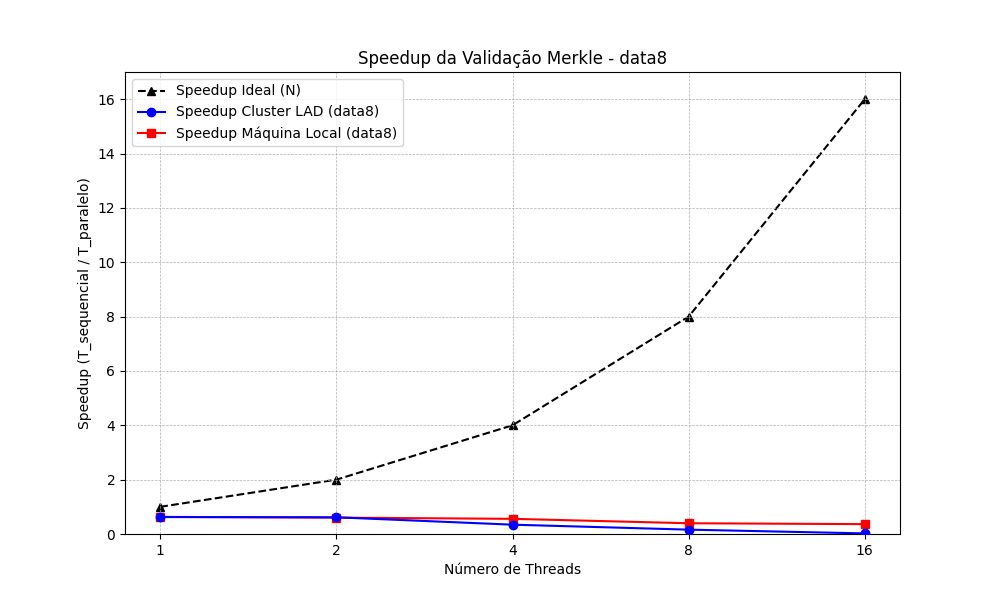
\includegraphics[width=0.8\textwidth]{graficos/speedup_data8.png}
    \caption{Gráfico de Speedup para o dataset `data8`.}
    \label{fig:speedup_data8}
\end{figure}

\begin{figure}[!htbp]
    \centering
    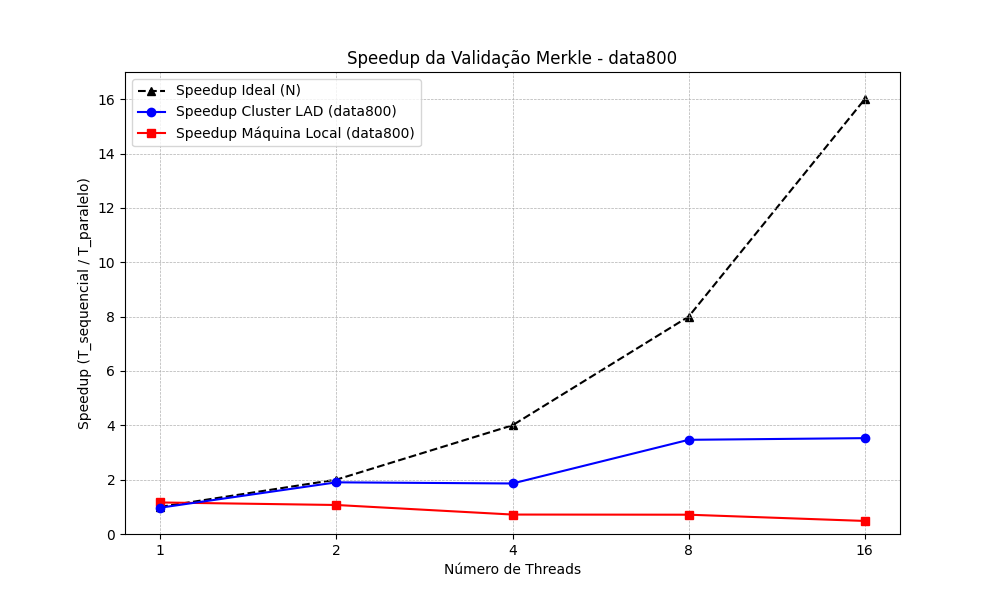
\includegraphics[width=0.8\textwidth]{graficos/speedup_data800.png}
    \caption{Gráfico de Speedup para o dataset `data800`.}
    \label{fig:speedup_data800}
\end{figure}

\begin{figure}[!htbp]
    \centering
    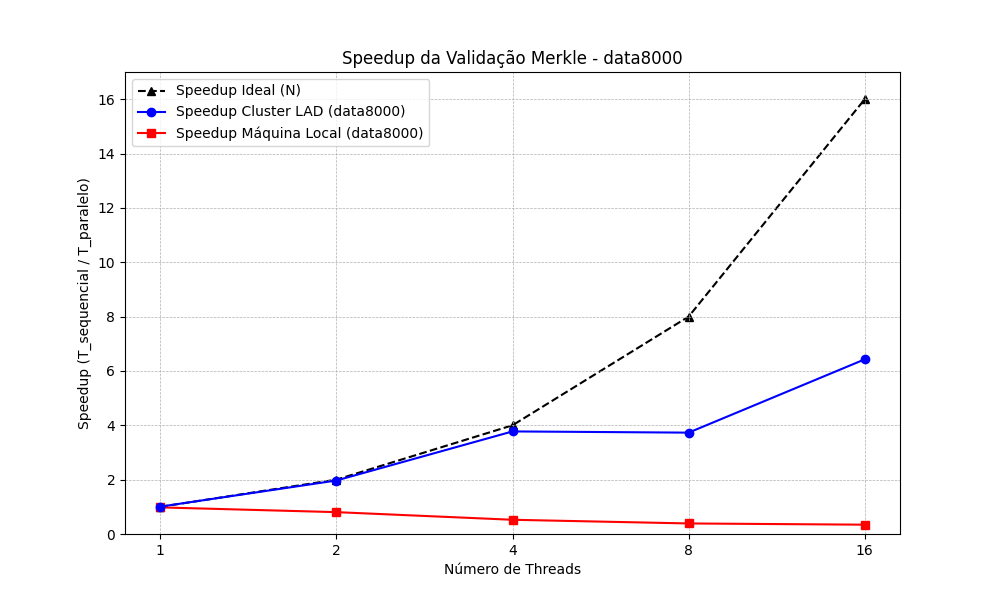
\includegraphics[width=0.8\textwidth]{graficos/speedup_data8000.png}
    \caption{Gráfico de Speedup para o dataset `data8000`.}
    \label{fig:speedup_data8000}
\end{figure}

\begin{figure}[!htbp]
    \centering
    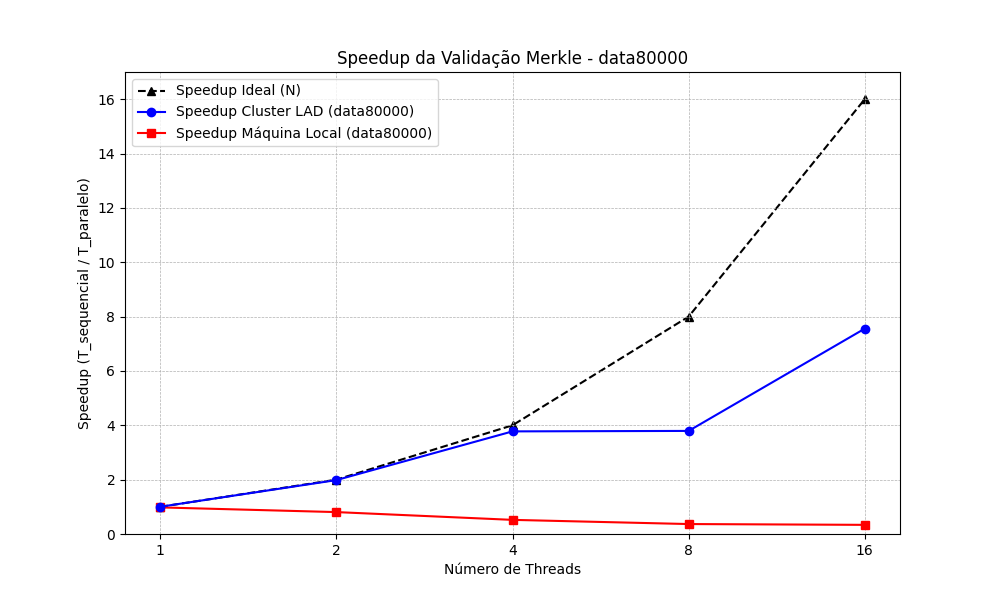
\includegraphics[width=0.8\textwidth]{graficos/speedup_data80000.png}
    \caption{Gráfico de Speedup para o dataset `data80000`.}
    \label{fig:speedup_data80000}
\end{figure}

% --- Apêndice C: Código Fonte Completo ---
\clearpage
\section{Código Fonte Completo}
\label{app:codigo}

% --- Listagem: merkle_validation_common.h ---
\lstinputlisting[
    caption={Arquivo Header Comum (\texttt{merkle\_validation\_common.h})},
    label={lst:common_h},
    inputencoding=utf8
]{merkle_validation_common.h}

\vspace{1em} % Espaço entre listagens

% --- Listagem: merkle_validation_utils.c ---
\lstinputlisting[
    caption={Funções Utilitárias (\texttt{merkle\_validation\_utils.c})},
    label={lst:utils_c},
    inputencoding=utf8
]{merkle_validation_utils.c}

\vspace{1em}

% --- Listagem: merkle_validation_sequential.c ---
\lstinputlisting[
    caption={Versão Sequencial (\texttt{merkle\_validation\_sequential.c})},
    label={lst:sequential_c},
    inputencoding=utf8
]{merkle_validation_sequential.c}

\vspace{1em}

% --- Listagem: merkle_validation_parallel.c ---
\lstinputlisting[
    caption={Versão Paralela com OpenMP (\texttt{merkle\_validation\_parallel.c})},
    label={lst:parallel_c},
    inputencoding=utf8
]{merkle_validation_parallel.c}


\end{document}
